\subsubsection{Project : Creating new Projects}
	Once a user has been successfully authenticated by the UPRM system, the user should be able to create a new project. On creation of a new project, the user will have to provide the following details:
	\begin{itemize}
		\item Name(or Title) of the new project.
		\item A short description of the new project.
		\item An overall project deadline.
		\item Optional project specific sub-deadlines to track progress. The default timeline will be from project creation date to overall project deadline and a 1\% progress.
	\end{itemize}
	\textbf{Pre-Conditions}
	\begin{itemize}
		\item User has to be successfully authenticated.
	\end{itemize}
	\textbf{Post-Conditions}
	\begin{itemize}
		\item A new project should be created.
		\item The new project information should be saved in a database.
	\end{itemize}
	
	\centerline{\fbox{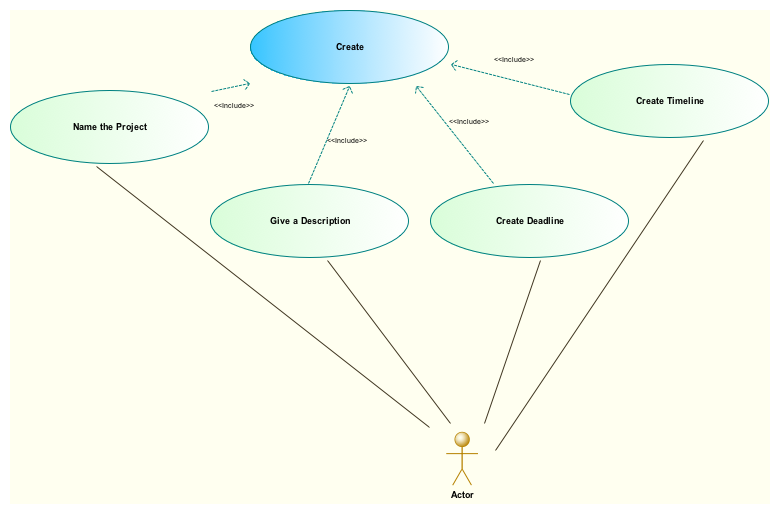
\includegraphics[width=\linewidth]{CRUD/uprm_create.png}}}